\documentclass[11pt]{report}
\usepackage{standalone}
\graphicspath{ {images/} }
\setcounter{tocdepth}{5}
\setcounter{secnumdepth}{5}
\usepackage{natbib}
\usepackage{bibentry}
\bibliographystyle{agsm}
\usepackage{etoolbox}
\setlength{\parindent}{0em}
\setlength{\parskip}{0.25em}
\usepackage[raggedright]{titlesec}
\usepackage{hyperref}
\usepackage{capt-of}
\patchcmd{\bibliography}{\section*}{\section}{}{}
\titlespacing*{\chapter}{0pt}{-40pt}{10pt}
\titleformat{\chapter}[block]{\normalfont\huge\bfseries}{\thechapter}{15pt}{}
\usepackage{rotating}
\usepackage[titletoc]{appendix}
\usepackage{pgfgantt}
\usepackage{graphicx, rotating, caption, lscape, threeparttable}% \usepackage{amsmath}
\usepackage{array}
\usepackage{pdflscape}
\usepackage{geometry}
\usepackage{listings}
\usepackage[T1]{fontenc}
\usepackage[bottom]{footmisc}
\usepackage{subcaption}
\usepackage{float}




\begin{document}
\chapter{Implementation}
\section{Software Stack Selection}

\subsection{Programming Language}
The System as analyzed in the specification requires a number of common computational tasks including web-scraping, natural language processing, machine learning, database interfacing and task execution handlers. To avoid reinventing the wheel within the scope of the system, the design decision of utilizing libraries where possible was taken. Libraries for the above-mentioned operations exist across popular programming languages however through further analysis Python became the obvious candidate. Python as a language promotes the integration of existing Python modules and `has an active supporting community of contributors and users that also make their software available for other Python developers to use under open source license terms'  \footnote{Python Modules accessible via https://docs.python.org/3/installing}.

\subsection{Framework}
The componentized system as highlighted in Figure \ref{fig:component} consists entirely of back-end components except for the singular visualizer front-end component. Due to the API nature of the back-end interfacing with the front-end, there was room to have a complete separation between the back-end and the front-end where a Python back-end would power a front-end framework that is completely detached from the business logic of the back-end system. However, the bulk of the requirements laid in the back-end and thus having a separate framework for the front-end could be argued to be overcomplicating the implementation of what is a well-structured System architecture. The design rationale was therefore taken to implement the back-end and front-end in a singular framework whilst upholding the design of having the business logic and API in the back-end allowing future extensibility of pulling the front-end into a separate framework at a later date if the System required it.
\\

Having decided on a singular framework for the system, the approach was taken to research and compare the top three python frameworks that would offer full stack capabilities along with a number of identified desirable quantities needed in the framework. Using the comparisons conducted in Table \ref{table:framework-comparison} and further research the framework decided upon was Django for it's out of the box capabilities and separate application support being most appropriate for the proposed solution (batteries included).
\\

\begin{tabular}{ |p{1.5cm}||p{2cm}|p{2cm}|p{2cm}|p{1.75cm}|p{1.75cm}|  }
 \hline
 \multicolumn{6}{|c|}{Full Stack Python Web Framework Comparison} \\
 \hline
 Name & Python Version Required & Separate Application Support & Templating & Batteries Included & Github Stars\\
 \hline
 Django & 3.X    & Yes &   Yes & Yes & 32,770\\
 Flask &   $\geq$ 3.3  & No & Yes & No & 34,207\\
 Pyramid & $\geq$ 3.4 & No &  Yes &  No & 2,700\\
 \hline
\end{tabular}
\captionof{table}{Python Framework Comparison \textbf{as of publishing date}}
\label{table:framework-comparison}

\section{System Architecture}
Through the implementation of the Python full-stack framework ``Django'', the system is encapsulated in a set of Python modules separated into ``applications'' that represent the high-level components of the system. Each application is registered within the system and contains a number of Python classes which are responsible for providing the component responsibilities that the application represents. The System also contains utility modules which are used across all the applications and therefore are available at the top level of the system. Along with applications, there are multiple configuration files and scripts that enable the remote execution of the system.

\subsection{Applications}
The applications provided by the system and the component that they represent are as follows:

\begin{itemize}
\item \textbf{classifiers}: representative of the classifier framework component.
\item \textbf{core}: representative of the visualizer component.
\item \textbf{tokenizer}: representative of the preprocessing framework component.
\item \textbf{scraper}: representative of the scraper component.
\end {itemize}

Each application contains a series of classes that provide the functionality required for the application and some Django specific classes for configuration (non-capitalized). If the application interfaces with the database it will contain a ``models.py'' file which are Django representations of the database tables that the application owns. Each application also contains a ``views.py'' file which also forms part of the visualizer component as each applications ``views.py'' file provides API endpoints that populate the template pages when requested.

\subsection{Dependency Injection}
The system contains two methods of dependency injection to provide the system access to third-party libraries of established code, it utilizes a python virtual environment to inject python libraries into the system for use within the back-end components of the system and nodejs is used to inject javascript and CSS libraries into the system for using within the front-end visualizer component of the system. On starting the system, the dependencies are copied over to the global ``static/'' folder from which they are globally accessible from within the system. The configuration files for dependency injection are \texttt{requirements.txt} (back-end injection) and \texttt{package.json} (front-end injection) which both contain a list of dependencies and there versions utilized by the system.
\\

\textit{N.B. Third party libraries that have been used without dependency injection have been clearly stated within the code using a header comment.}

\section{Database Implementation}
The System contains two database implementations, the live production PostgreSQL database hosted via AWS and the auxiliary test SQLite database used for integration testing of the system. The implementation of database structure required the translation of each model in the entity relationship diagrams into Django Models such that the System could then utilize the built-in object-relational mapping (ORM) tool to easily access database records without the need for SQL. Django handles the database management of the system with changes to the models occurring through \textit{South Migrations} which are then propagated to the database. The entities from the physical entity-relationship diagram were translated into Django Models with each attribute from the entity being a field of the representative Django Model. Through translation of the data models, a number of constraints were also implemented to enforce the data integrity within the database. For illustration purposes the translation of the Tweet entity can be seen in Figure \ref{fig:model-translation}

\begin{center}
  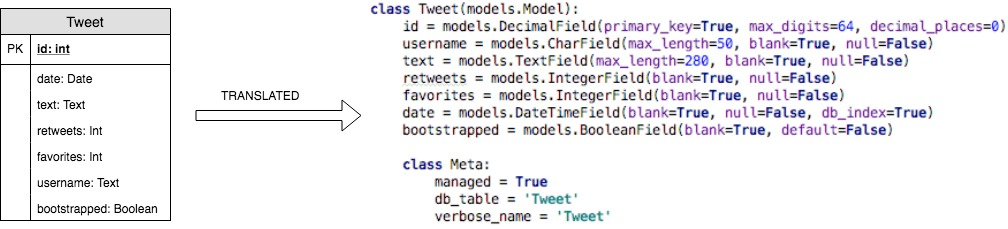
\includegraphics[width=16cm]{images/model-translation.jpg}
  \captionof{figure}{Data Model Translation.}
  \label{fig:model-translation}
\end{center}
\clearpage

\section{System Features}
The System features that were outlined in the proposed specification have their implementations listed below.

\subsection*{Tweet Collection}
The scraper application hosts two interfaces with Twitter for the collection of tweets. Having two application product interfaces (that communicate with Twitter) for the collection of tweets allows for the collection of \textbf{historic} and \textbf{current (in real-time)} tweets.

\subsubsection*{Historic Scraper}
The system integrates the existing third party tweet collector named ``GetOldTweets-python'' \footnote{GetOldTweets-python accessible via https://github.com/Jefferson-Henrique/GetOldTweets-python} that allows for the backdating of tweets older than two weeks. It does this by manually scraping the JSON of the twitter advanced search timeline using the requested dates, languages and hashtags as filter criteria. The historic interface was amended to work within the Django framework and optimized using the system's concurrency utilities to allow for thread pool execution of the extraction of tweets from the JSON as well as asynchronous saving of tweet objects to the database.

\subsubsection*{Real Time Scraper}
The system integrates the existing third party tweet collector named ``Tweepy'' \footnote{Tweepy accessible via http://www.tweepy.org/} that allows for the collection of tweets in real time i.e. as they are posted. Tweepy allows the system to communicate with twitters firehose (tweet access) provider ``gnip'' and request access to real time tweets for a specified language and hashtags.
\\

Tweepy enables a connection between the client application and gnip to be established, then queries the streaming API with the filter criteria resulting in the delivery of tweets to the client application as they are posted and upon close of the connection attempts to retry connecting until a new connection is established and the collection restarts. The raw tweet JSON objects are placed in a Redis message broker to process the saving of tweets asynchronously via a celery application. The asynchronous processing is key to the operating of real-time collection as gnip delivers tweets from a fixed size queue which only holds tweets for a limited time before disposing of them. Celery (an asynchronous task executor) then processes the receive tweet task in which the raw tweet JSON is converted into a tweet model object and then saved to the database.

\begin{center}
  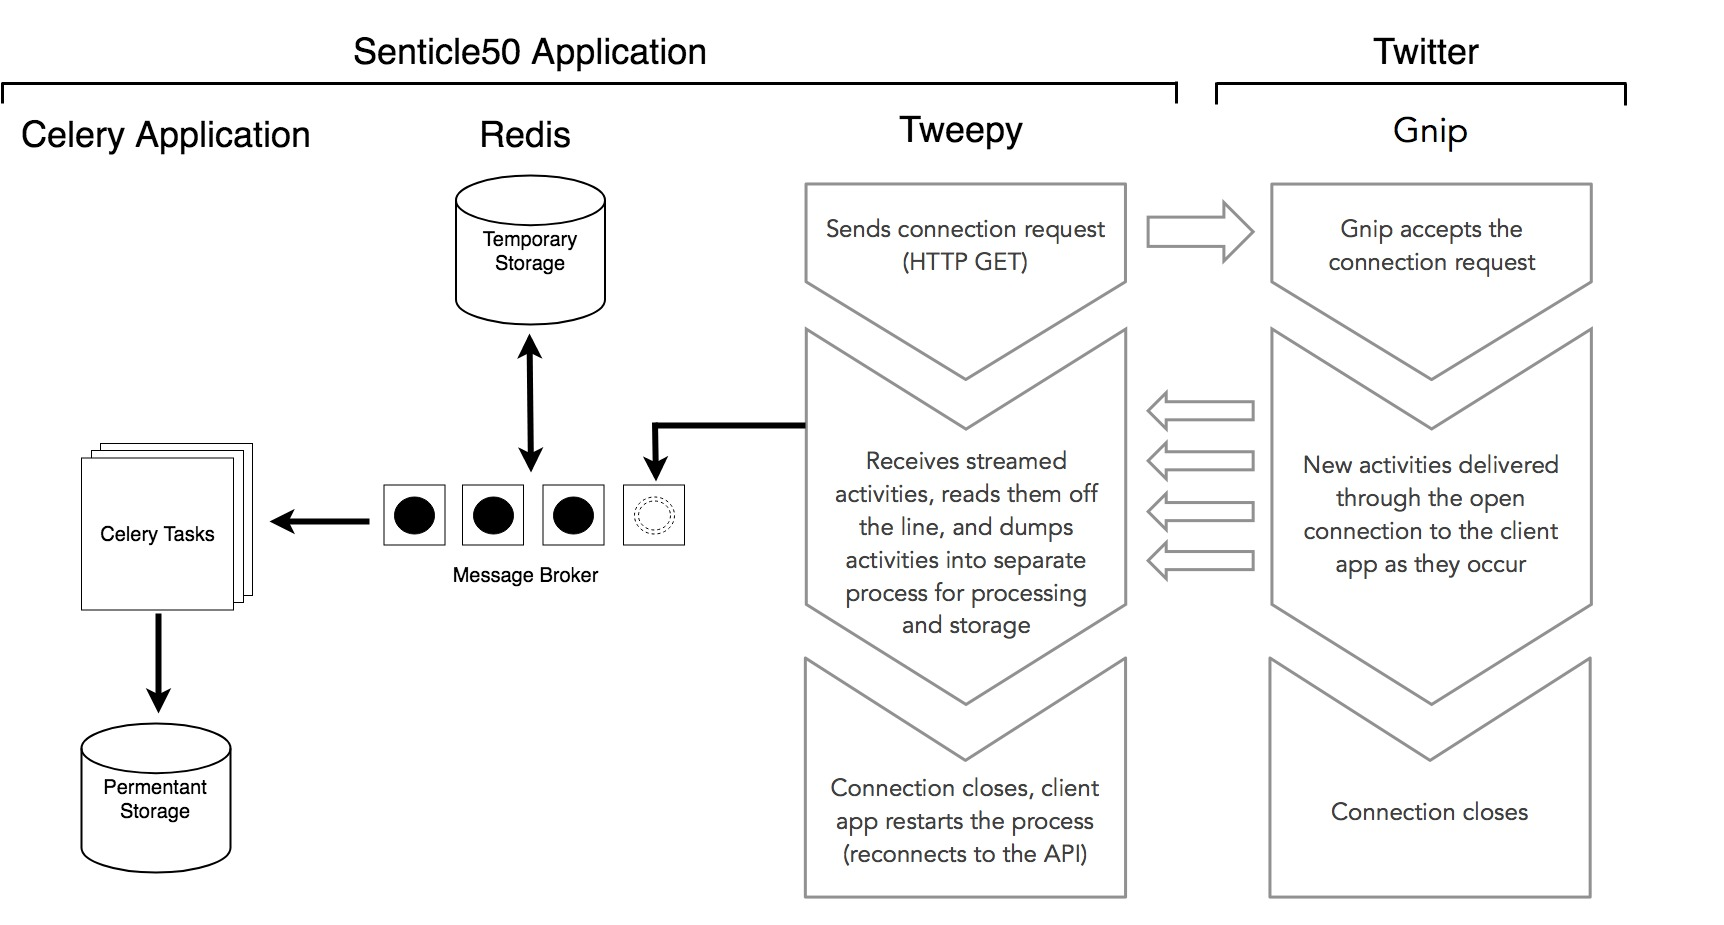
\includegraphics[width=\textwidth]{images/real-time-tweet-collection.jpg}
  \captionof{figure}{Real-Time Tweet Collection \protect\footnotemark.}
  \label{fig:syspipe}
\end{center}

\footnotetext{Modified Image accessible via http://support.gnip.com/articles/consuming-streaming-data.html}

\subsection*{Tweet Tokenization}
The tokenizer application implements the preprocessing step of tweet classification, it manipulates the raw text of tweet objects and converts tweets into a ``Tokenized Form''.
\\

Each Tweet is converted into a string of ``Tokens'' through a series of tokenization steps that utilize regular expressions and the natural language toolkit to accomplish this. A tweet's raw text will therefore go through the following steps in order

\begin{enumerate}
\item All text is lowered in case.
\item Twitter Mentions are replaced e.g. @UserMention.
\item Hashtags are removed e.g. \#Example.
\item Twitter ``RT'' symbol for retweet is removed.
\item Extra whitespace is removed
\item URL's are removed e.g. http://url.com
\item Stop words are removed e.g. his/her.
\item Punctuation is removed e.g. ! , / ' ( )
\item Remaining text is split into an array of tokens (words)
\item Words are stemmed to reduce dimensionality of feature set e.g. running -> run
\item Final tokens are joined back together as a token string.
\end{enumerate}

\subsection*{Tweet Classification}

The classifiers application implements the classification framework component of the system. The set of implemented classifier classes contains the  \texttt{CombinationClassifier}, \texttt{KerasClassifier}, \texttt{StringContainsClassifier} and \texttt{StringEndClassifier}. Each of the the implemented classifiers classifies tweets against a model which is passed in as an attribute when instantiating the classifiers as mentioned in the Design. The classifiers application exposes two main services that can be interacted with, the \texttt{ClassifierService} for classifying tweets on a one tweet per classification basis and the \texttt{BatchClassifierService} for classifying larger groups of tweets on a batch basis. The classifiers application also provides two registry classes that implement the registry pattern discussed in the design; the \texttt{ClassifierRegistry} and \texttt{RealTimeClassifierRegistry}.

\subsubsection*{Model Architecture}
The models that utilize a neural network i.e. the \texttt{Naive Brexit Model} and \texttt{Sentiment Model} have been created using the Neural Network library Keras. Each of the models convert the tokenized tweets into a padded vector of 140 length (that can represent the new max length of 280 characters within tweets). Each entry in the vector therefore represents the presence of a word using the index of the word from the tokenized feature set of the top five thousand words found in the training set of the model. Utilizing this structure in the model therefore takes the context (order) of the words as well as the presence of the words for learning patterns of order unique to the classes through the convolutional layers defined within the network. See the experiments application \texttt{management/commands/} folder for the model neural network structures.

\subsubsection*{Classifier Architecture}
The architecture of classifiers has each of the classifiers implement the interface of a Classifier superclass. The set of implemented classifiers within the classifiers application are all subclasses of the abstract base class \texttt{Classifier}. Through the subclass relationship they are required to implement the abstract methods defined within ``Classifier'' and thus the interface relationship is enforced (See Listing .

\clearpage
\begin{center}
\begin{lstlisting}
from abc import ABC, abstractmethod

class Classifier(ABC):

    @abstractmethod
    def __init__(self, model_to_load):
        pass

    @abstractmethod
    def classify(self, text, model_parameters):
        pass

    @abstractmethod
    def classify_batch(self, texts, model_parameters):
        pass

    @abstractmethod
    def get_classifier_name(self):
        pass
        
@classifier
class KerasClassifier(Classifier):

    def __init__(self, model_to_load):
        ...

    def classify(self, text, model_parameters):
        ...

    def classify_batch(self, texts, model_parameters):
        ...

    def get_classifier_name(self):
        ...

\end{lstlisting}
\captionof{lstlisting}{An example of Classifier interface utilization.}
\end{center}

\clearpage

\subsubsection*{Classifier Registries}
The aforementioned classifier registries are populated by the scripts \texttt{RegisterClassifiers} and \texttt{RegisterRealTimeClassifiers} located in the scripts folder within the system wide configuration folder of \texttt{brexit/brexit/}. Each registry is an instantiation of a \texttt{Singleton} base class thus providing system wide access to the available classifiers after being populated on startup of the system.

\begin{center}
\begin{lstlisting}
class ClassifierRegistry(Singleton):
 
    def _init(self):
        self.classifiers = {}

    def get_registered_classifiers(self):
        return self.classifiers

    def add(self, classifier_name, classifier):
        if classifier_name not in self.classifiers:
            self.classifiers[classifier_name] = classifier

    def get(self, classifier_name):
        if classifier_name in self.classifiers:
            return self.classifiers[classifier_name]

        raise ValueError(`Classifier not found in classifier registry')
\end{lstlisting}
\captionof{lstlisting}{ClassifierRegistry.py class implementation}
\end{center}

The ClassifierRegistry provided by the classifiers application allows for a service to be generic by dynamically pulling the class implementation of the configured classifier and instantiating it. 

\begin{center}
\begin{lstlisting}
classifier = ClassifierRegistry().get(config['classifier_name'])
\end{lstlisting}
\captionof{lstlisting}{Usage of ClassifierRegistry}
\end{center}

The \texttt{RegisterClassifiers} script is executed first and populates the \texttt{ClassifierRegistry} with each of the available classifiers within the system that end in ``Classifier''. For a classifier to be registered within the \texttt{ClassifierRegistry} it is required to have the \textit{classifier decorator} which allows for the classifier to be added to registry upon import.

\begin{center}
\begin{lstlisting}
def classifier(cls):
    classifier_registry = ClassifierRegistry()
    classifier_registry.add(cls.get_classifier_name(), cls)
    return cls
    
@classifier
class KerasClassifier(Classifier):
    ...
    @staticmethod
    def get_classifier_name():
        return "KerasClassifier"

\end{lstlisting}
\captionof{lstlisting}{Usage of  ``classifier'' decorator}
\end{center}

After the \texttt{ClassifierRegistry} is populated the \texttt{RegisterRealTimeClassifiers} script begins to populate the \texttt{RealTimeClassifierRegistry} with the json classification configuration files that contain the boolean flag ``is\textunderscore real \textunderscore time'' that is true. It is the configuration files that are contained in the \texttt{RealTimeClassifierRegistry} that are utilized in the real time classification of tweets.

\subsection*{Visualisation}
The application core and the \texttt{views.py} files contained in the rest of the applications together make up the visualizer component of the system. The visualizer component as highlighted in Design is split into pages, with each page begin reachable by the navigation bar (visible at the top of the page) except for the classifier-analysis page which is accessed via buttons within the analysis page and thus is the only second depth page in the visual system. The visual component utilizes bootstrap for css conformity and cross browser/device layout support, jQuery for user interactions and D3 for the analysis pictorial visualisations displayed on the classifier-analysis page. 

\subsubsection*{API}
The system has a number of configured url paths which are registered in the system within \texttt{urls.py} files. These url paths are regular expressions that match the url of a given request and handle the execution of that url accordingly. If the url does not match any of the registered url paths within the system Django returns a page-not-found exception (HTTP 404) and renders the 404.html page found within the \texttt{templates/} folder. On the successful match of a url a \texttt{views.py} endpoint is called to render a template and JSON context that holds the data for the template to display.

\subsubsection*{Template Pages}
The System uses Django's built-in templating feature to populate pages where the information is displayed dynamically i.e. data displayed on the page is not static. The templating structure consists of a base template \texttt{index.html} that defines the overall layout of the website and includes the elements of the site which are viewable regardless of page e.g. navigation header and footer. The base template defines a body section which each child template page then extends with the content of that page. Each template page serves one url except the classifier-analysis page which serves four url's; one for each displayable time unit. Using a single template for the classifier-analysis page allows the rendering of four unique views of the page each of which has dynamic data populated through various permutations of the parameters classifier type and time period.
\\

The final set of viewable implemented pages as outlined in the Design are as follows; \texttt{home.html}, \texttt{analysis.html}, \texttt{classifier-analysis.html}, \texttt{data.html} and \texttt{about.html}.

\begin{figure}[H]
        \begin{subfigure}[b]{0.30\textwidth}
                
\includegraphics[width=\linewidth, height = 3cm]{images/home.png}
                \caption{home page}
                \label{fig:gull}
        \end{subfigure}%
        \hfill
        \begin{subfigure}[b]{0.30\textwidth}
                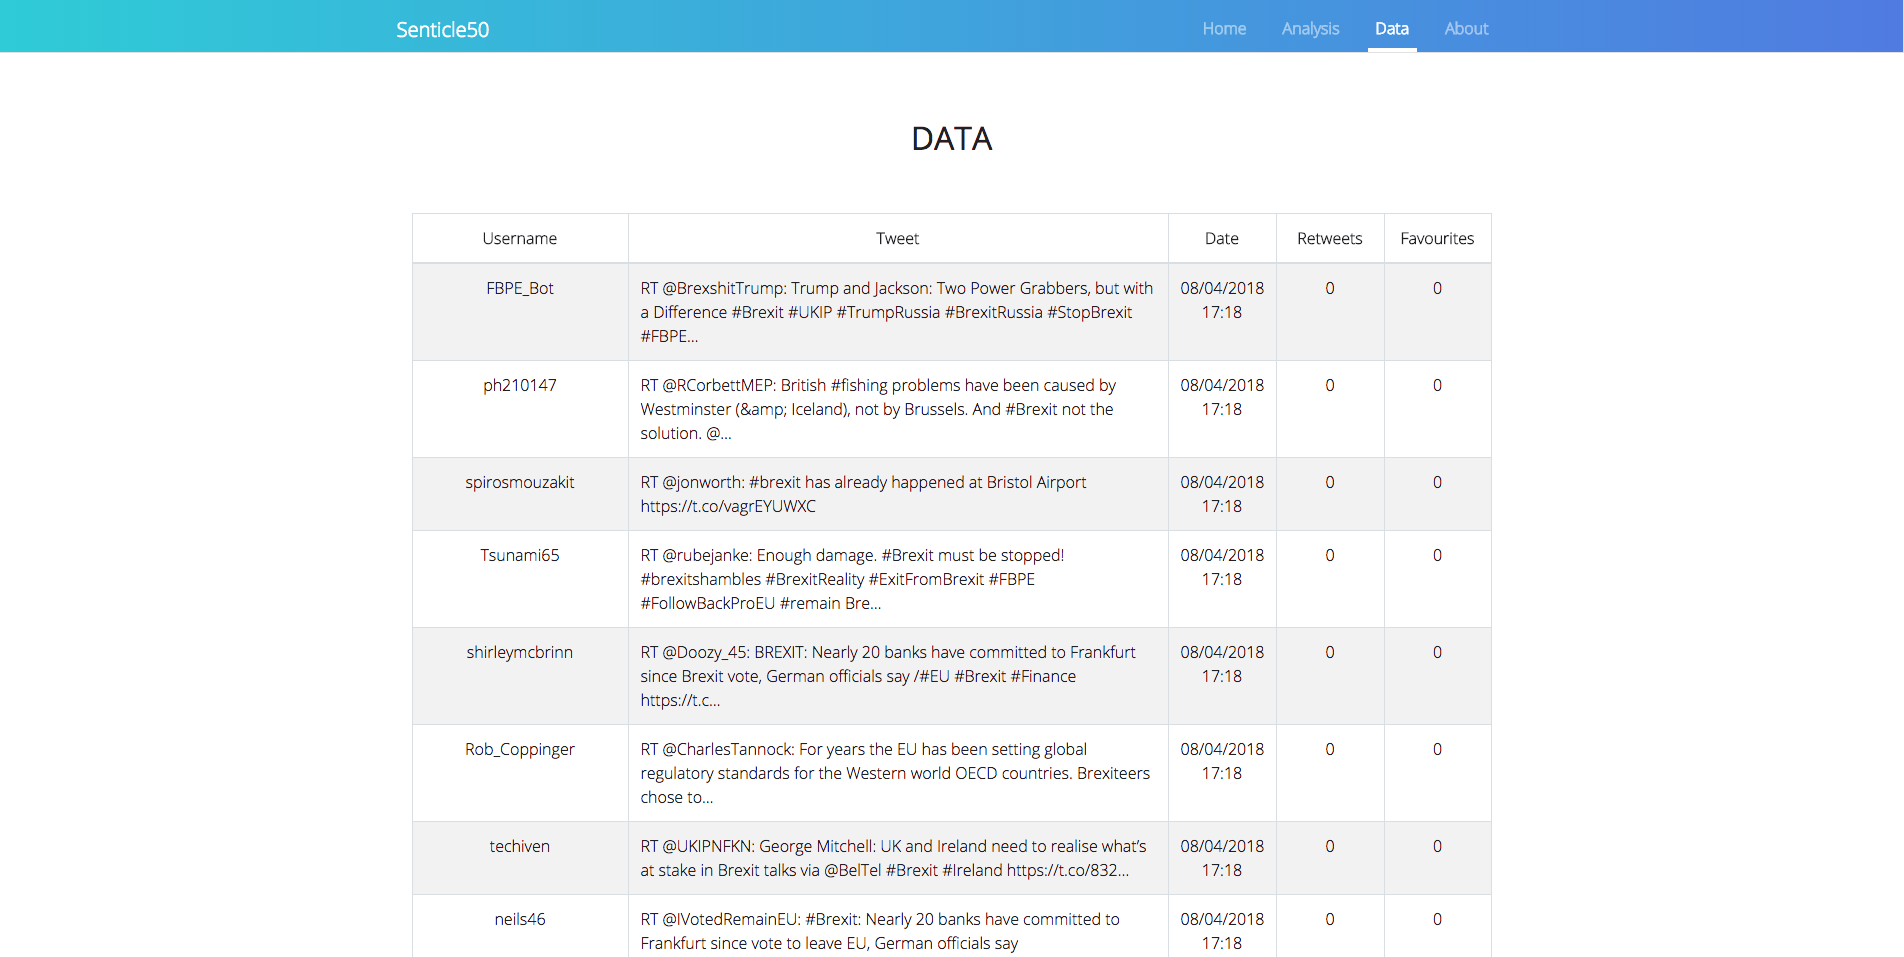
\includegraphics[width=\linewidth, height = 3cm]{images/data.png}
                \caption{data page}
                \label{fig:gull2}
        \end{subfigure}%
        \hfill
        \begin{subfigure}[b]{0.30\textwidth}
                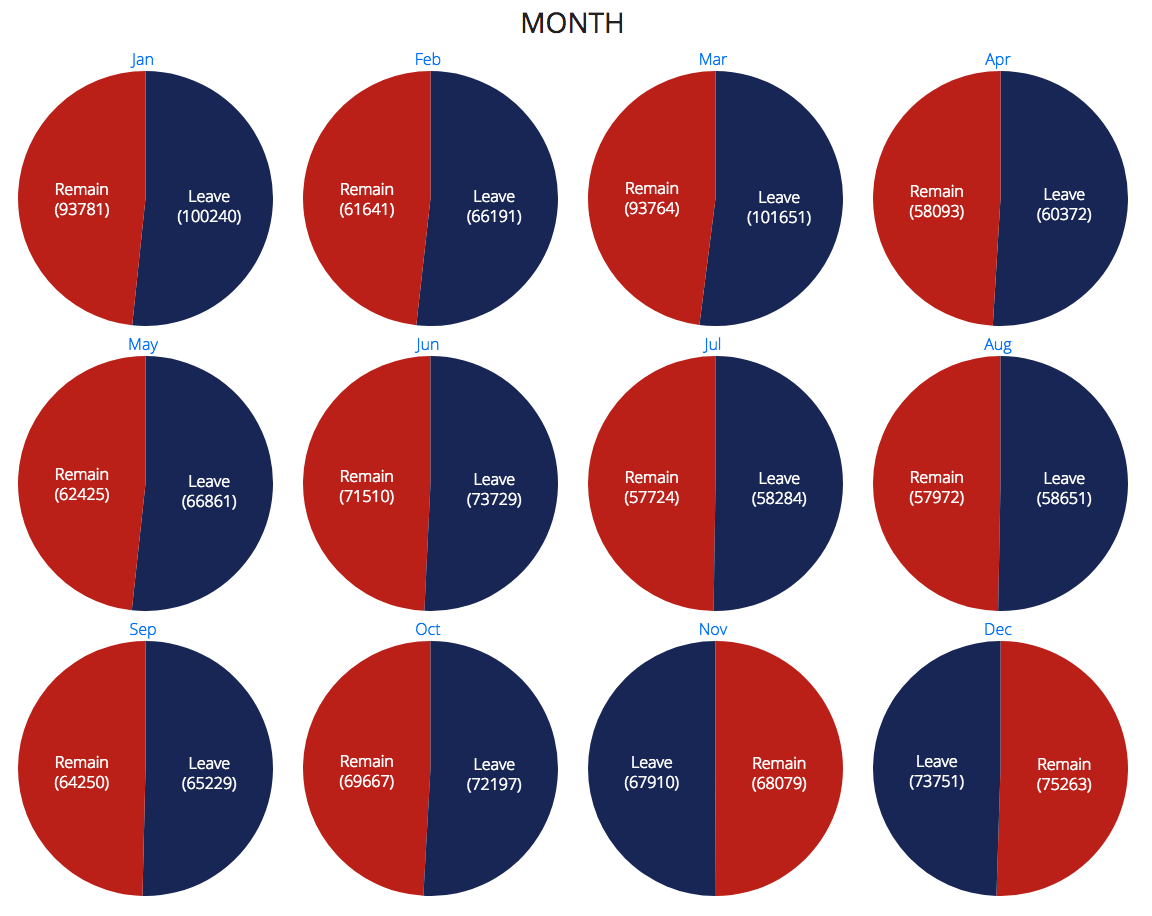
\includegraphics[width=\linewidth, height = 3cm]{images/analysis.png}
                \caption{analysis}
                \label{fig:tiger}
        \end{subfigure}%

        \caption{System Website Screenshots.}\label{fig:screenshots}
\end{figure}

\subsection*{Automation}
The automation of the system is the flow between all of the components within the system. The System pipeline outlined in the Design has been implemented through a series of scripts  that configured remotely on the server. The remote server uses a process control system named Supervisor to ensure all of the automated tasks are running. The system also uses a scheduled cron job to classify the new tweets it has received every five minutes.
\\

The system automation is split into two tasks: the collection and tokenization of a tweet as well as the classification and visualisation of those tweets. As mentioned in the tweet collection system feature implementation, asynchronous tasks are used to convert the real-time collected tweets into tweet models. After conversion to a tweet model the tweet is also tokenized. The collection and tokenization of the tweets requires the running of the system  and the Celery (asynchronous executor) application. To ensure both of these system's are running a Supervisor configuration was enabled for each of commands to run the two systems required. It was found that the classification of tweets on a one tweet per classification basis was inefficient for real time classification as Keras required a lock when asked to predict a class given a sample, hence batch classification and visualisation was chosen to be a task of it's own. The batch classification and visualisation classifies and updates the composite visual objects required for visualisation on the tweets which haven't yet been classified today, this task runs every five minutes on a scheduled cron job.


\enlargethispage{\baselineskip}
\section{Deployment}
\label{sec:deployment}
For the deployment of the system onto the remote virtual private server the continuous delivery environment \textit{Jenkins} was used. Jenkins as a tool allows for the automation of tasks through the specification of a delivery pipeline. The System utilizes a \texttt{JenkinsFile} which specifies the continuous delivery pipeline consisting of a Build, Test and Deploy step (see Figure \ref{figure:deliverypipe}). Upon running the System's pipeline, Jenkins handles the pulling of the System's GitLab repository itself after which it is the Build and Deploy steps of the delivery pipeline which is required for deployment of the System via Jenkins. The Build step first installs a clean environment for the System to run in ensuring that all dependencies are injected, the static front-end files are generated and that the System can be built i.e. that it compiles. After a successful build the Deploy step handles across a secured ssh connection to the remote server; the removal of the old system, the copying of the new system files via the secure copy protocol and the restarting of the system through supervisor commands. Upon successful execution of the delivery pipeline the System is backup within seconds containing the new changes which had been committed to the System's GitLab repository prior to running the delivery pipeline. 
\\

\textit{N.B. If any steps within the delivery pipeline fail, the deployment of the system is aborted with Jenkins displaying the source of error thus preventing a faulty system from being deployed onto the live production server}.

\begin{center}
  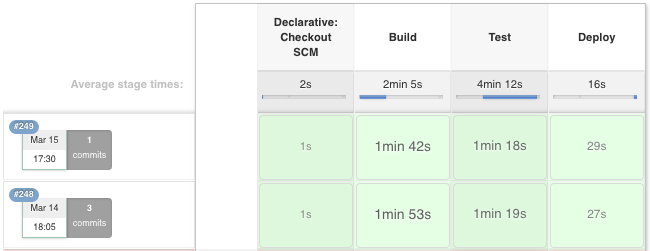
\includegraphics[width=0.9\textwidth]{images/delivery-pipeline.png}
  \captionof{figure}{Jenkins view of the Continuous Delivery Pipeline.}
  \label{figure:deliverypipe}
\end{center}

\end{document}